% TEMPLATE.TEX
%
% Time-stamp: <2013-03-26 11:09 olenz>
%
% This is an extensively documented LaTeX file that shows how to
% produce a good-looking document with current LaTeX (11/2012).
%
% IMPORTANT!
%
%   Some obsolete commands and packages
% ----------|-------------------------------
% obsolete  |     Replacement in LATEX 2ε
% ----------|-------------------------------
%           | local            global/switch
% ----------|-------------------------------
% {\bf ...} | \textbf{...}     \bfseries
%     -     | \emph{...}       \em
% {\it ...} | \textit{...}     \itshape
%     -     | \textmd{...}     \mdseries
% {\rm ...} | \textrm{...}     \rmfamily
% {\sc ...} | \textsc{...}     \scshape
% {\sf ...} | \textsf{...}     \sffamily
% {\sl ...} | \textsl{...}     \slshape
% {\tt ...} | \texttt{...}     \ttfamily
%     -     | \textup{...}     \upshape
%
% DON'T USE \\ TO MAKE LINEBREAKS, INSTEAD JUST LEAVE A BLANK LINE!
%
\RequirePackage[l2tabu,orthodox]{nag} % turn on warnings because of bad style
\documentclass[a4paper,10pt,bibtotoc]{scrartcl}
%
\usepackage[bottom=3.5cm, top=2cm]{geometry}
%%%%%%%%%%%%%%%%%%%%%%%%%%%%%%%%%%%%
% KOMA CLASSES
%%%%%%%%%%%%%%%%%%%%%%%%%%%%%%%%%%%%
%
% The class "scrartcl" is one of the so-called KOMA-classes, a set of
% very well done LaTeX-classes that produce a very European layout
% (e.g. titles with a sans-serif font).
%
% The KOMA classes have extensive documentation that you can access
% via the commands:
%   texdoc scrguide # in German
%   texdoc scrguien # in English
%
%
% The available classes are:
%
% scrartcl - for "articles", typically for up to ~20 pages, the
%            highest level sectioning command is \section
%
% scrreprt - for "reports", typically for up to ~200 pages, the
%            highest level sectioning command is \chapter
%
% scrbook  - for "books", for more than 200 pages, the highest level
%            sectioning command is \part.
%
% USEFUL OPTIONS
%
% a4paper  - Use a4 paper instead of the default american letter
%            format.
%
% 11pt, 12pt, 10pt
%          - Use a font with the given size.
%
% bibtotoc - Add the bibliography to the table of contents
%
% The KOMA-script classes have plenty of options to modify

% This allows to type UTF-8 characters like ä,ö,ü,ß
\usepackage[utf8]{inputenc}

\usepackage[T1]{fontenc}        % Tries to use Postscript Type 1 Fonts for better rendering
\usepackage{lmodern}            % Provides the Latin Modern Font which offers more glyphs than the default Computer Modern
\usepackage[intlimits]{amsmath} % Provides all mathematical commands

\usepackage{hyperref}           % Provides clickable links in the PDF-document for \ref
\usepackage{graphicx}            % Allow you to include images (like graphicx). Usage: \includegraphics{path/to/file}

% Allows to set units
\usepackage[ugly]{units}        % Allows you to type units with correct spacing and font style. Usage: $\unit[100]{m}$ or $\unitfrac[100]{m}{s}$

% Additional packages
\usepackage{url}                % Lets you typeset urls. Usage: \url{http://...}
\usepackage{breakurl}           % Enables linebreaks for urls
\usepackage{xspace}             % Use \xpsace in macros to automatically insert space based on context. Usage: \newcommand{\es}{ESPResSo\xspace}
\usepackage{xcolor}             % Obviously colors. Usage: \color{red} Red text
\usepackage{booktabs}           % Nice rules for tables. Usage \begin{tabular}\toprule ... \midrule ... \bottomrule

% Source code listings
\usepackage{listings}           % Source Code Listings. Usage: \begin{lstlisting}...\end{lstlisting}
\lstloadlanguages{python}
\definecolor{lightpurple}{rgb}{0.8,0.8,1}

\lstset{
stepnumber=1,
numbersep=5pt,
numberstyle=\small\color{black},
basicstyle=\ttfamily,
%keywordstyle=\color{black},
%commentstyle=\color{black},
%stringstyle=\color{black},
frame=single,
tabsize=4,
language = python,
backgroundcolor=\color{black!5}}

\usepackage{float}

\begin{document}

\titlehead{Simulation Methods in Physics II \hfill SS 2020}
\title{Report for Worksheet 2: Properties of water from quantum mechanical and atomistic simulation}
\author{Markus Baur and David Beyer}
\date{\today}
\maketitle

\tableofcontents

\section{Short Questions --Short Answers}
\begin{itemize}
\item \textbf{A1}: Water molecules consist of one oxygen atom (O) and two hydrogen atoms (H). Because oxygen has a much higher electronegativity (i.e a tendency to attract bond electrons towards itself) than hydrogen, water molecules exhibit positive partial charges at the hydrogen atoms and negative partial charges at the oxygen atoms. A dipole moment arises (i.e the molecules are polar) because of the non-linear (bent) molecular structure.

\item \textbf{A2}: A hydrogen bond is a weak bond (compared to covalent or ionic bonds) which arises between a (partially positively charged) hydrogen atom (as part of a molecule) and partially negatively charged atom like oxygen (e.g. in water, i.e also part of a molecule). Hydrogen bonds can be intermolecular (e.g. in water) or intramolecular (e.g. in DNA or proteins).

\item \textbf{A3}: The H--O--H angle in water molecules is about 104.45$^\circ$.\footnote{https://en.wikipedia.org/wiki/Properties\_of\_water, accessed on May 8 2020, 20:00} Hydrogen bonds in water have a typical length of 1.97$\r{A}$.\footnote{http://chemistry.elmhurst.edu/vchembook/161Ahydrogenbond.html, accessed on May 8 2020, 20:00}

\item \textbf{A4}: 
\end{itemize}

\section{Quantum Mechanical Calculation of Water}
\subsection{Quantum Mechanical Calculation of Water}
\subsection{Ab Initio Molecular Dynamics Simulation of Water Dimer}
\subsection{Infrared Spectroscopy}

\section{Atomistic Simulation of Water}
\subsection{Running the Simulations}
We performed atomistic simulations of 216 water molecules using GROMACS and three different water models (SPCE, SPCE/E and TIP3P). The temperature was set to $T=300\,\mathrm{K}$ and the simulations were run for 250000 time steps of size $\Delta t = 2\,\mathrm{ps}$

\subsection{Analysis}
\subsubsection*{Radial Distribution Function}
\autoref{fig:fig_gromacs_1} -- \autoref{fig:fig_gromacs_3} show the calculated radial distribution functions for the different water models.

\begin{figure}[h]
\centering
 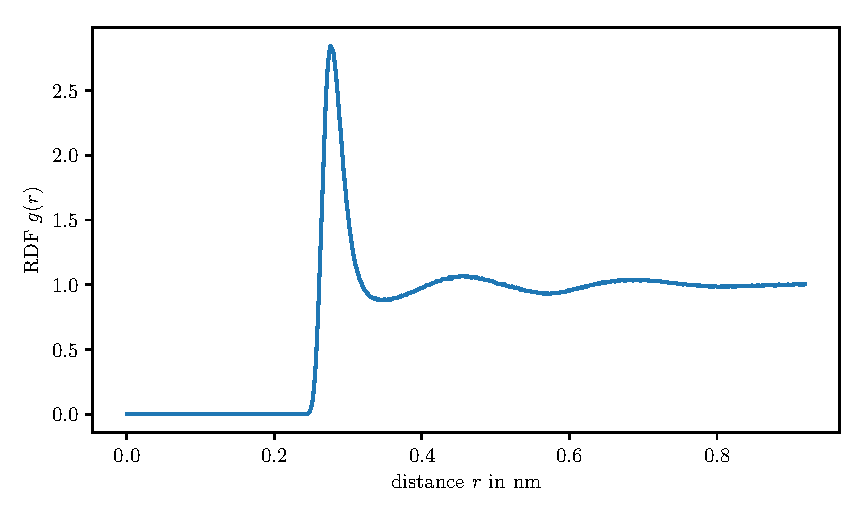
\includegraphics[width=0.8\textwidth]{RDF_SPC.pdf}
 \caption{Radial distribution function for the SPC water model.}
 \label{fig:fig_gromacs_1}
 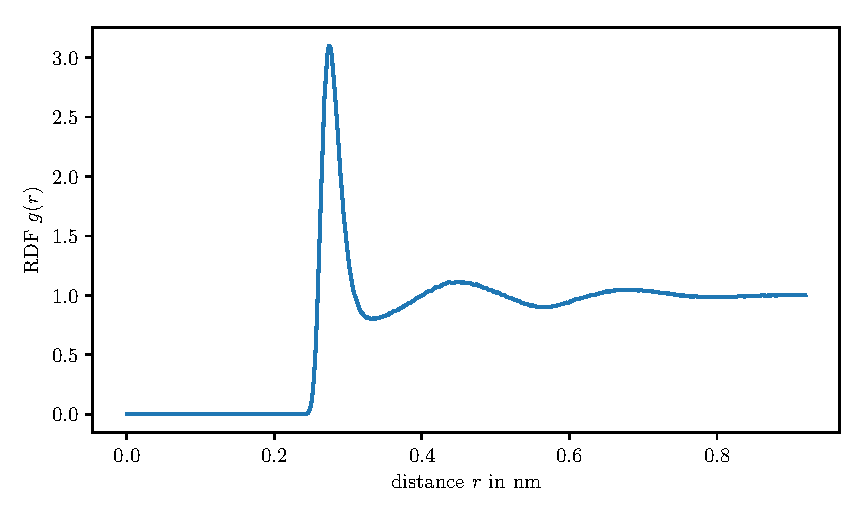
\includegraphics[width=0.8\textwidth]{RDF_SPCE.pdf}
 \caption{Radial distribution function for the SPCE water model.}
 \label{fig:fig_gromacs_2}
 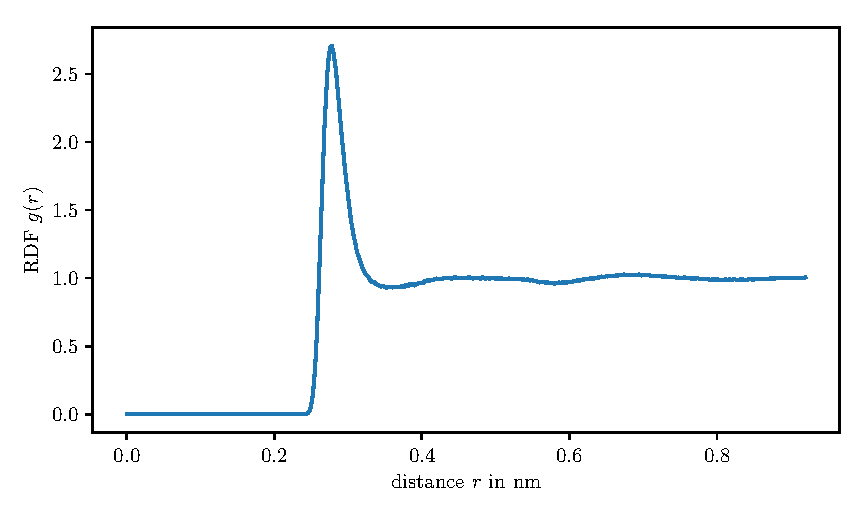
\includegraphics[width=0.8\textwidth]{RDF_TIP3P.pdf}
 \caption{Radial distribution function for the TIP3P water model.}
 \label{fig:fig_gromacs_3}
\end{figure}

\subsubsection*{Hydrogen Bond Analysis}
The number of hydrogen bonds per water molecule for the three different water models is shown in \autoref{tab1}.

\begin{table}[h]
\centering
\caption{Average number of hydrogen bonds per water molecule for different water models.}
\begin{tabular}{@{}cc@{}}
\toprule
water model & avg. number of H-bonds \\ \midrule
SPC         &          1.73                 \\
SPCE        &          1.80               \\
TIP3P       &          1.67                 \\ \bottomrule
\end{tabular}
\label{tab1}
\end{table}

\subsubsection*{Mean Square Displacement and Diffusion Coefficient}
\autoref{fig:fig_gromacs_4}--\autoref{fig:fig_gromacs_6} show plots of the mean square displacement which was computed for the different water models.

\begin{table}[h]
\centering
\caption{Computed diffusion coefficients for the different water models}
\begin{tabular}{@{}cc@{}}
\toprule
water model & diffusion coefficient $D$ in $10^{-5}\,\mathrm{cm}^2\cdot \mathrm{s}^{-1}$ \\ \midrule
SPC         &          3.7948 $\pm$ 0.1089                 \\
SPCE        &          2.2704 $\pm$ 0.1190            \\
TIP3P       &          5.0608 $\pm$       0.3821    \\ \bottomrule
\end{tabular}
\label{tab1}
\end{table}


\begin{figure}[h]
\centering
 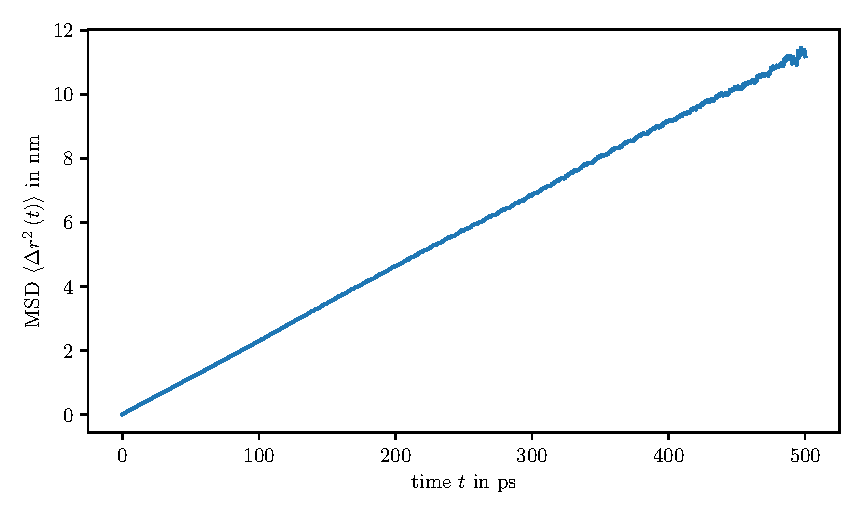
\includegraphics[width=0.8\textwidth]{MSD_SPC.pdf}
 \caption{Mean square displacement for the SPC water model.}
 \label{fig:fig_gromacs_4}
 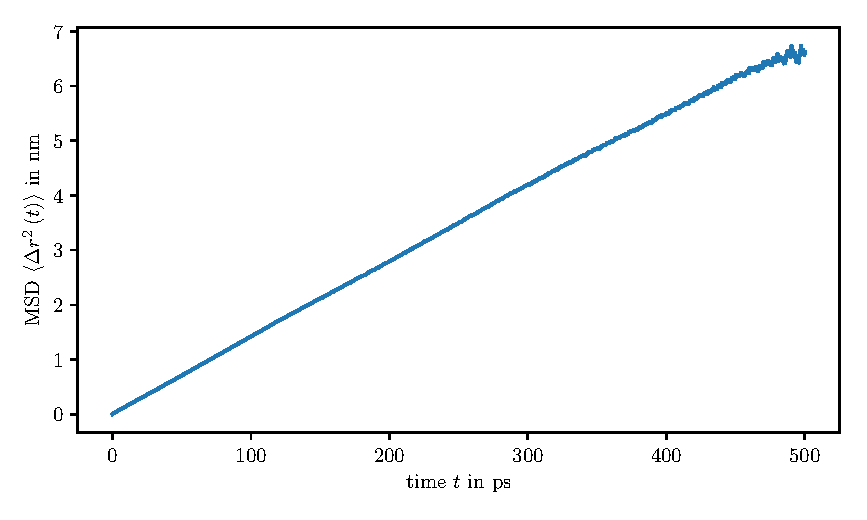
\includegraphics[width=0.8\textwidth]{MSD_SPCE.pdf}
 \caption{Mean square displacement for the SPCE water model.}
 \label{fig:fig_gromacs_5}
 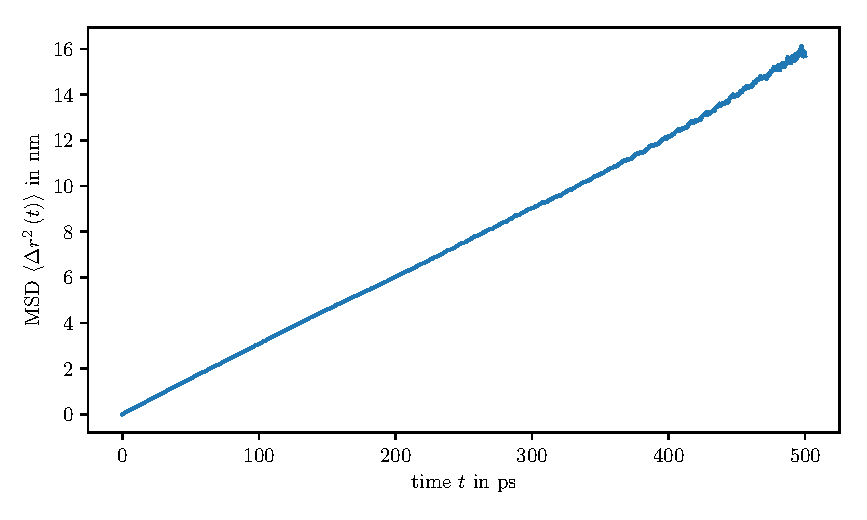
\includegraphics[width=0.8\textwidth]{MSD_TIP3P.pdf}
 \caption{Mean square displacement for the TIP3P water model.}
 \label{fig:fig_gromacs_6}
\end{figure}

\begin{figure}[h]
\centering
 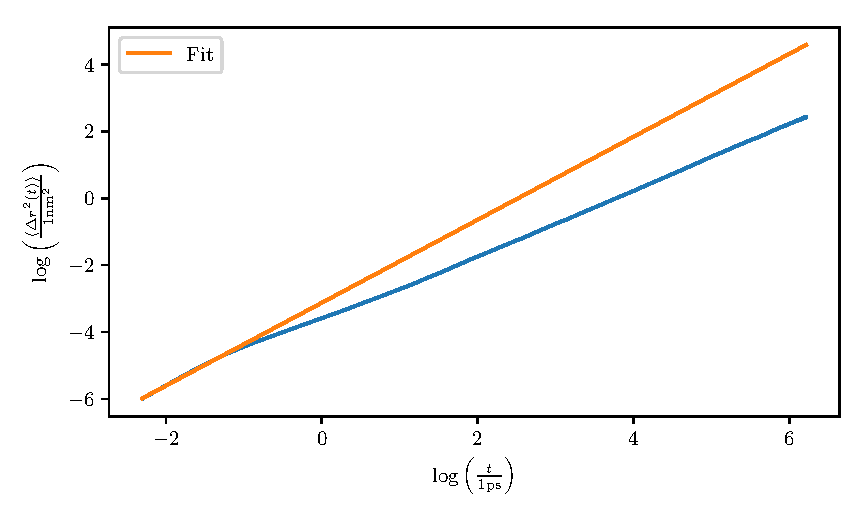
\includegraphics[width=0.8\textwidth]{MSD_SPC_LOG.pdf}
 \caption{Log-log plot of the mean square displacement for the SPC water model.}
 \label{fig:fig_gromacs_7}
 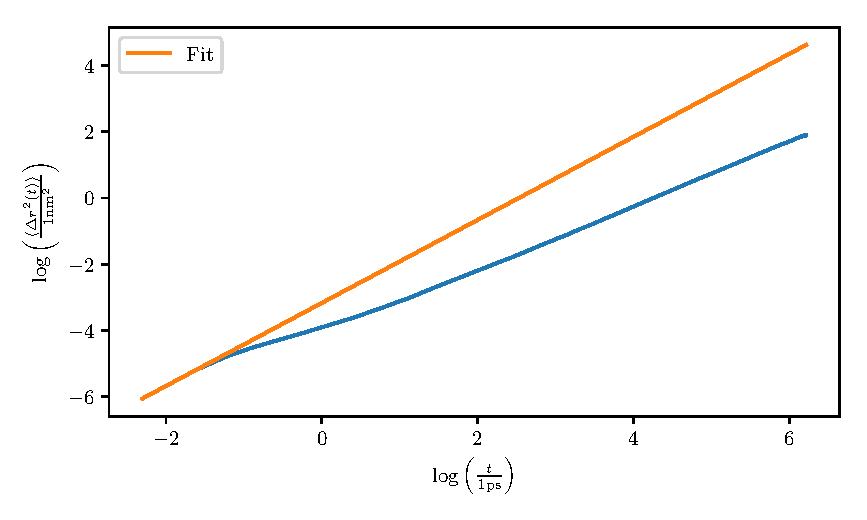
\includegraphics[width=0.8\textwidth]{MSD_SPCE_LOG.pdf}
 \caption{Log-log plot of the mean square displacement for the SPC water model.}
 \label{fig:fig_gromacs_8}
 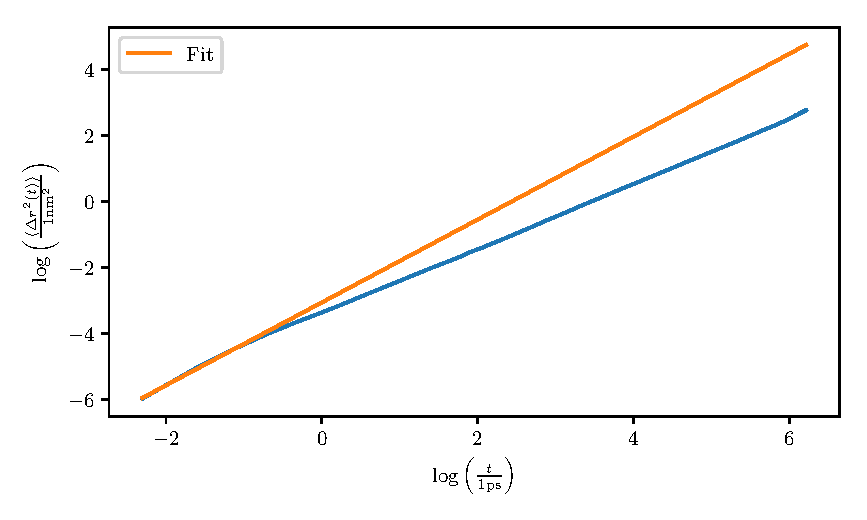
\includegraphics[width=0.8\textwidth]{MSD_TIP3P_LOG.pdf}
 \caption{Log-log plot of the mean square displacement for the SPC water model.}
 \label{fig:fig_gromacs_9}
\end{figure}

\end{document}
